\subsection{Architektur}\label{subsec:architektur}

\begin{wrapfigure}{r}{.5\textwidth}
	\centering
	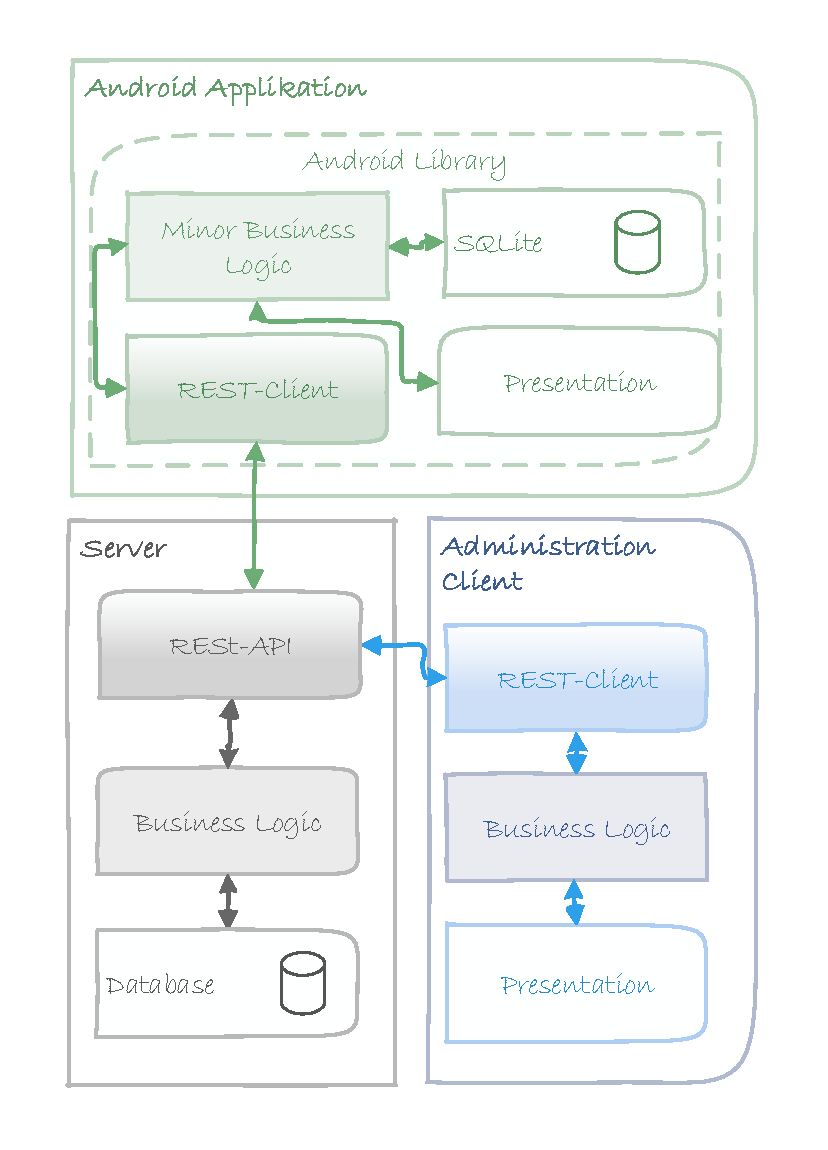
\includegraphics[width=\linewidth]{img/architecture_draft}
	\caption{Architektur des Frameworks.}
	\label{fig:architektur_entwurf}
\end{wrapfigure}
Das Framework ist in drei Komponenten unterteilt: Server, Android Bibliothek und ein Client für Testleiter~/~Administratoren.

Der Aufbau der Komponenten ist in Abbildung \ref{fig:architektur_entwurf} dargestellt.
Die Kommunikation zwischen den Komponenten erfolgt per \ac{HTTP} und ein \ac{REST} - \ac{API}.
Der Server nutzt zur Datenhaltung eine Datenbank, auf welche durch die Geschäftslogik zugegriffen wird.

Der Administrations-Client dient zum Verwalten der Tests, Aufgaben und Benutzer, sowie zum Einsehen von Ergebnissen bereits durchgeführter Testsitzungen.
Er besitzt keine eigene Datenhaltung und erhält sämtliche Daten vom Server über einen \ac{REST}-Client.

Die Android Bibliothek kommuniziert auch über einen \ac{REST}-Client mit dem Server.
Um Testsitzungen auch ohne Internetverbindung oder allgemein der Verbindung zum Server durchführen zu können, speichert die Android Bibliothek Tests, Aufgaben und die gesammelten Daten von Testsitzungen lokal zwischen.
Diese werden bei der nächsten Verbindung mit dem Server an diesen übertragen.